\subsubsection{Primer 1 - Dijagonale matrica}

\large{1. Opis zadatka}
\normalsize

Napraviti Client-Server aplikaciju koja će komunicirati na TCP portu X (gde je $X = broj\ indeksa/24 + 2000$) i omogućavati klijentima da igraju igru dijagonala matrica uz pomoć kockica.

\large{2. Opis igre}
\normalsize

Svaki igrač ima dve kockice koje imaju \textbf{N} strana i tabelu predstavljenu kao \textbf{$N\times N$} matricu. Igra se odvija po potezima i u svakom potezu igrač baca obe kockice istovremeno. Brojevi koji se dobiju nakon jednog bacanja kockica predstavljaju kooridnate matrice. Ukoliko se koordinate nalaze na glavnoj dijagonali tabele igrač popunjava to polje i dobija bonus potez. Ukoliko se ne nalaze na glavnoj dijagonali, protivniku se šalje poruka da je on na potezu. Pobednik igre je igrač koji prvi popuni glavnu dijagonalu matrice.

Serveru se sa konzole unosi broj N koji označava broj strana kockica i veličinu matrice ($N\times N$):

\begin{figure}[H]
    \centering
    
\includegraphics[width=0.5\textwidth]{Slike/DM/DM_Velicina_matrice.png}
    \label{fig:dm_velicina}
\end{figure}

\large{3. Specifikacija zadatka}
\normalsize

Aplikacija treba da podržava konekciju sa dva klijenta koji će predstavljati igrača 1 i igrača 2. Nakon pokretanja aplikacije, klijent treba da se konektuje na server i započne igru porukom “start”. Nakon poslate poruke, klijent čeka povratnu poruku od servera koja potvrđuje početak igre. Server nakon povezivanja prvog klijenta čeka da se konektuje i drugi, nasumično određuje ko prvi igra i javlja klijentu koji je na potezu da može započeti svoj potez.

Klijent koji je na potezu šalje serveru poruku “baci kockice” i od njega dobija dva nasumična broja u formatu {X,Y} koji predstavljaju brojeve dobijene bacanjem prve i druge kockice. Klijent kod sebe čuva tabelu kao matricu i ispisuje je nakon svakog bacanja kako bi mogao da prati stanje igre.

Ukoliko je klijent dobio broj na dijagonali, recimo {3,3}, potrebno je obeležiti dobijeno polje na matrici sa znakom “o”. Ukoliko je dobio brojeve koji nisu na dijagonali, recimo {1,3}, potrebno je obeleziti ih znakom “x” na matrici. Matrica se klijentu prikazuje nakon svakog bacanja. Svaki put kada klijent popuni polje na matrici, server obaveštava drugog klijenta da je njegov protivnik popunio polje na dijagonali. Svaki put kada klijent popuni polje na dijagonali dobija bonus potez, onog trenutka kada ne dobije polje koordinate dijagonale drugi klijent preuzima potez.

Klijenta koji popuni sva polja na dijagonali server proglašava za pobednika i obaveštava o tome oba klijenta.

\begin{figure}[H]
    \centering
    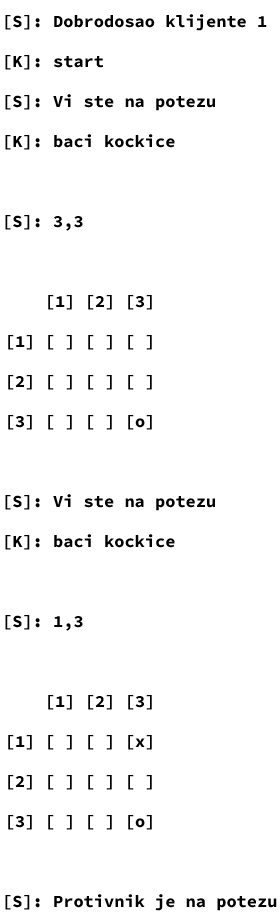
\includegraphics[width=0.25\textwidth]{Slike/DM/DM_Igrac_prvi.png}
    \caption*{Primer komunikacije servera i klijenta koji igra prvi}
    \label{fig:dm_prvi}
\end{figure}

\begin{figure}[H]
    \centering
    
\includegraphics[width=0.25\textwidth]{Slike/DM/DM_Igrac_drugi.png}
    \caption*{Primer komunikacije servera i klijenta koji igra drugi}
    \label{fig:dm_drugi}
\end{figure}